\documentclass[a4paper]{article}
\usepackage[scale=0.85]{geometry}
\usepackage{titling}
\usepackage{minted}
\usepackage{amsmath,amsfonts}
\usepackage{xcolor}
\usepackage{braket}
\usepackage{bm}
\usepackage{tensor}
\usepackage{cleveref}
% \usepackage{MnSymbol}
\usepackage{mhchem}
\usepackage{graphicx}

\usemintedstyle{vs}
\definecolor{bg}{rgb}{0.95,0.95,0.95}
\setminted{bgcolor=bg,linenos,breaklines}

\allowdisplaybreaks[4]

\makeatletter
\renewcommand{\maketitle}{%
    %   \sffamily
    \begin{flushleft}
    \sffamily
      {\Large\bfseries\@title\par}%
      \medskip
      {\large\course\par}%
      \medskip
      {\@date\par}%
    \end{flushleft}
     \begin{flushright}%
      {\@author\quad ID: \id\\}
      {\itshape \inst\\}
      {Email: \ttfamily\email}
   \end{flushright}%
   \rule{\textwidth}{1pt}\vspace*{2pc}%
}
\makeatother

\def\tr{\operatorname{tr}}


\title{Homework}
\author{Xue Chen}
\date{December 2022}

\def\course{Ultracold Atomic Physics}
\def\inst{Institute for Advanced Study, Tsinghua University}
\def\id{2022311901}
\def\email{chenx22@mails.tsinghua.edu.cn}

\begin{document}

\maketitle

\def\ahf{\alpha_{\mathrm{hf}}}
\def\muB{\mu_{\mathrm{B}}}
\def\gS{g_{\mathrm{S}}}
\def\muN{\mu_{\mathrm{N}}}
\def\gI{g_{\mathrm{I}}}

\section*{Problem 1.8}
\paragraph{} Considering a time-dependent Hamiltonian
\begin{equation}
    \hat{H} = \omega \hat{F_z} + B_0 \cos(\omega _0t) \hat{F_x},
\end{equation}
show that when $\omega_0$ is close to $\omega$, by rotating wave approximation, the Hamiltonian can become a time-independent one as
\begin{equation}
    \hat{H} = \Delta \hat{F_z} + \frac{B_0}{2} \hat{F_x}
\end{equation}
where $\Delta$ = $\omega - \omega_0$.
\paragraph{Solution:} 
Rewrite the Hamiltonian
\begin{equation}
    \hat{H} = \omega \hat{F_z} + \frac{B_0}{2}(e^{i\omega_0 t}+e^{-i\omega_0 t})\hat{F_x} 
\end{equation}
Using the unitary transformation$\hat{u}=e^{-i\omega_0 t \hat{F_z}/\hbar}$, and the formula 
\begin{equation}
    e^{\hat{A}} \hat{B} e^{-\hat{A}} = \hat{B} + [\hat{A},\hat{B}] + \frac{1}{2!}[\hat{A},[\hat{A},\hat{B}]]+...+\frac{1}{n!}[\hat{A},[\hat{A}...,[\hat{A},\hat{B}]...]+...   
\end{equation}
we get 
\begin{equation}
    \hat{u}^{\dag} \hat{F_x} \hat{u} = \hat{F_x}\cos(\omega_0 t)-\hat{F_y} \sin(\omega_0 t)
\end{equation}
take this bake to the Hamiltonian and expand the trigonometric functions by Euler formula, we get
\begin{equation}
    \hat{u}^{\dag} \hat{H} \hat{u} = \omega \hat{F_z} + \frac{B_0}{4} [(e^{2i\omega_0 t}+e^{-2i\omega_0 t}+2)\hat{F_x} + (e^{2i\omega_0 t}+e^{-2i\omega_0 t})\hat{F_y}
\end{equation}
by rotating wave approximation, the terms with $2\omega_0$ frequency can be dropped. Meanwhile, the transformation is time dependent, so the final results should be $\hat{H} \to \hat{u}^{\dag} \hat{H} \hat{u} + i\hbar (\partial_t \hat{u}^{\dag})\hat{u}$, the second term gives $-\omega_0 \hat{F_z}$
\begin{equation}
    \hat{H} \to \Delta \hat{F_z} + \frac{B_0}{2} \hat{F_x}
\end{equation}



\def\ahf{\alpha_{\mathrm{hf}}}
\def\muB{\mu_{\mathrm{B}}}
\def\gS{g_{\mathrm{S}}}
\def\muN{\mu_{\mathrm{N}}}
\def\gI{g_{\mathrm{I}}}

\section*{Problem 2.1}
\paragraph{} Calculate the scattering length for a three-dimensional square well interaction potential $V(r) = 0$ for $r>r_0$, $V(r) = -V_0$ for $r_0 > r>0$ with $V_0>0$ and $V(r) = \infty$ for r=0. Discuss how the scattering length changes as a function of $V_0$, and discuss when the binding energy satisfies the relation $E = -\hbar^{2}/(2\Bar{m} {a_s}^2)$
\paragraph{Solution:} 
Because the potential is spherical symmetric, we can expand the wave function in the relative coordinate in terms of angular momentum partial waves:
\begin{equation}
    \Psi(\bm{r}) = \sum_l \frac{\chi_{kl}(r)}{k r}\mathcal{P}_l(\cos(\theta))
\end{equation}
At low energy, the interaction effect is dominated by the s-wave channel, i.e. $l = 0$, so we can consider this special case only. The Schrodinger equation is:
\begin{equation}
    -\frac{\hbar^2}{2m}\nabla^2 \chi_k(r) + V(r) \chi_k(r) = E \chi_k(r)
\end{equation}
In the regime $r>r_0$, the wave function can be written as:
\begin{equation}
    \chi_k(r) \propto \sin(k r + \delta_k) \approx \sin(\delta_k) + k r \cos(\delta_k) \propto 1-\frac{r}{a_s},
\end{equation}
so the scattering length just equal to the node of the wave function at $r>r_0$.
When $0<r<r_0$, the wave function can be solved as:
\begin{equation}
    \chi_k(r) = \sin(\sqrt{\frac{2V_0m}{\hbar^2}}r)
\end{equation}
The slope should be the same at $r = r_0$,
% so we have $-\frac{1}{a_s} \propto \sqrt{\frac{2V_0m}{\hbar^2}} \cos( \sqrt{\frac{2V_0m}{\hbar^2}}r_0)$
% When a_s close to 0, higher order should be considered. So the slope is not a good tool while node does.
so the wave function at $r>r_0$ is just extension cord and the node is $a_s$. As the slope at $r_0$ varies periodical (not strictly) with $V_0$, the node as well as $a_s$ goes from infinity to negative infinity repeatedly. 
\paragraph{}
When the binding energy $E = -\hbar^{2}/(2\Bar{m} a_s^2)$, the $a_s$ should be positive. When $s_s \to \infty$, the binding energy $\to 0$. As $V_0$ increases and $a_s$ decreases, the binding energy increases. This means the bound state becomes deeper and can not be described by this low energy assumption.









\def\ahf{\alpha_{\mathrm{hf}}}
\def\muB{\mu_{\mathrm{B}}}
\def\gS{g_{\mathrm{S}}}
\def\muN{\mu_{\mathrm{N}}}
\def\gI{g_{\mathrm{I}}}

\section*{Problem 2.2}
\paragraph{} Calculate the scattering length for a three-dimensional hard core potential $V(r) = 0$ for $r>r_0$, $V(r) = -V_0$ for $r_0 > r>0$ with $V_0>0$ and $V(r) = \infty$ for r=0. Discuss how the scattering length changes as a function of $V_0$ and the difference from the square well potential above.
\paragraph{Solution:} 
In the regime $0<r<r_0$, the wave function is:
\begin{equation}
    \chi_k(r) = \sinh{\sqrt{\frac{2V_0m}{\hbar^2}}r}
\end{equation}
This is the hyperbolic sine function which strictly increase monotonically. The node as well as $a_s$ increase from $-\infty$ to $r_0$ and stay at $r_0$ for bigger $V_0$.









\section*{Problem 2.3}
Show that for a finite range interaction $V(r) \simeq 0$ for $r>r_0$, the phase shift for the $l$th partial wave $\delta_l \propto k^{2l+1}$
\paragraph{Solution:} 
In the $r>r_0$ regime, the function to be solved can be written as: 
\begin{equation}
    \frac{d^{2} u_{kl}}{dr^2} - \frac{l(l+1)}{r^2} u_{kl} + k^2 u_{kl} = 0
\end{equation}
with $E = \frac{\hbar^2k^2}{2\Bar{m}}$, and the radial wave function $\chi_{kl} = \frac{u_{kl} }{r}$.

In the $r\to\infty$ limit, the function becomes 
\begin{equation}
    \left[\frac{d^{2}}{dr^2} + k^2\right] u_{kl} \approx 0
\end{equation}
and the general solution is
\begin{equation}
    u_{kl}(r) \approx A e^{ikr} + B e^{-ikr}
\end{equation}
which can be regarded as superposition of incoming wave and outgoing wave. Because of the conservation of probability, the modula of $A$ and $B$ should be the same. Then:
\begin{equation}
    u_{kl}(r) \approx C \sin \left(kr-l\frac{\pi}{2}+\delta_l\right)
\end{equation}
The reason we insert the $l\frac{\pi}{2}$ is that for free particle the $\delta_l=0$.

So the large-distance behavior of the radial wave function is:
\begin{equation}
    \chi_{kl} \approx C\frac{e^{-ikr}e^{il\pi/2}-e^{ikr}e^{-il\pi/2}e^{2i\delta_l}}{2ikr}
\end{equation}

On the other hand, the wave function at $r>r_0$ regime can be written in the basis of spherical harmonic functions. Then it is therefore a linear combination of $j_l(kr)P_l(\cos\theta)$ and $n_l(kr)P_l(\cos\theta)$. With the spherical Hankel functions defined as
\begin{equation}
    h_l^{(1)} = j_l +in_l, h_l^{(2)} = j_l-in_l
\end{equation}
the radial wave function is 
\begin{equation}
    \chi_{kl} = c_l^{(1)}h_l^{(1)} +c_l^{(2)}h_l^{(2)}
\end{equation}
At large r limit, we have
\begin{equation}
    h_l^{(1)} \to \frac{e^{i\left(kr-l\pi/2\right)}}{ikr}, h_l^{(2)} \to \frac{e^{-i\left(kr-l\pi/2\right)}}{ikr}
\end{equation}
Taking this into (19) and compare with (17), we have 
\begin{equation}
    \chi_{kl} \propto j_l(kr)\cos\delta_l - n_l(kr)\sin\delta_l
\end{equation}

In this specific potential, there should be $\chi_{kl}(R) =0$. Therefore the condition for the phase shift should be
\begin{equation}
    \tan\delta_l = \frac{j_l(kR)}{n_l(kR)}
\end{equation}
In the low energy limit, which means $kR\ll1$, we have
\begin{equation}
    \begin{aligned}
        &j_l(kr) \simeq \frac{(kr)^l}{(2l+1)!!} \\
        &n_l(kr) \simeq -\frac{(2l-1)!!}{(kr)^{l+1}}
    \end{aligned}
\end{equation}
and then 
\begin{equation}
    \tan\delta_l =\frac{-(kR)^{2l+1}}{(2l+1)!!(2l-1)!!}
\end{equation}
Because $kR\ll1$, $\tan\delta_l \approx \delta_l$, so we get
\begin{equation}
    \delta_l \propto k^{2l+1}
\end{equation}
\section*{Problem 3.1}
Discuss the Bose-Einstein condensation temperature for free bosons at one and two dimensions.
\paragraph*{Solution:}
The density of bosons on each mode obays the Bose-Einstein distribution
\begin{equation}
    n_k = \frac{1}{e^{\left(\varepsilon _k - \mu\right) /k_BT}-1}
\end{equation}
For free bosons we have $\varepsilon_k = \frac{\hbar^2k^2}{2m}$. To let BEC occure, the chemical potential $\mu(T_c)=0$. 

In 1D, the conservation of the number of particles becomes
\begin{equation}
    N = \frac{L}{2\pi}\sum _k \frac{1}{\exp\left({\frac{1}{k_BT_c}\frac{\hbar^2k^2}{2m}}\right)-1}
\end{equation}
With the thermal de-Brogile wavelengh defined as 
\begin{equation}
    4\pi\frac{\hbar^2}{2m\lambda ^2} = k_BT
\end{equation}
and change the summation into integral, we have
\begin{equation}
    N = \frac{L}{2\pi}\int_{0}^{\infty} dk  \frac{1}{e^{(k\lambda_c)^2/4\pi}-1} = \frac{L}{2\pi \lambda_c}\int_{0}^{\infty} dx \frac{1}{e^{x^2/4\pi}-1}
\end{equation}
When $x \to 0$, the component in the integral approximates to $\frac{4 \pi}{x^2} $, leading the integral diverges.

For 2D, in the same way, we have
\begin{equation}
    N = \frac{S}{(2\pi)^2}\int_{0}^{\infty} 2\pi k dk  \frac{1}{e^{(k\lambda_c)^2/4\pi}-1} = \frac{S}{2\pi \lambda_c^2}\int_{0}^{\infty} dx \frac{x}{e^{x^2/4\pi}-1}
\end{equation}
The integral can be written as $\int_{0}^{\infty}dx \frac{1}{2}\frac{1}{e^{x/4\pi}-1}$, which also diverges when $x \to 0$.

In conclusion, the BEC temperature for the free bosons at one and two dimensions is zero. Or, at 1D and 2D, the free bosons do not condensate. 
\section*{Problem 3.2}
Calculate the two-body density matrix $\rho(\mathbf{r},\mathbf{r'})$ for noninteracting bosons above and below the Bose-Einstein condensation temperature.
\paragraph*{Solution:}
The two-body density matrix is defined as 
\begin{equation}
    \rho(\bm{r}_1, \bm{r}_2, \bm{r}'_1, \bm{r}'_2) = \braket{\hat{\Psi} ^{\dagger}(\bm{r}_1) \hat{\Psi }^{\dagger}(\bm{r}_2) \hat{\Psi}(\bm{r}'_1)\hat{\Psi}(\bm{r}'_2)}
\end{equation}
Under the situation $\bm{r}_1 \approx \bm{r}_2 \approx \bm{r}$ and $\bm{r}'_1 \approx \bm{r}'_2 \approx \bm{r}'$, we have
\begin{equation}
    \rho(\bm{r} , \bm{r}') \approx \sum_i N_i \psi ^*_i(\bm{r}) \psi_i(\bm{r}')
\end{equation}

Above the BEC temperature, in all modes the occupation number is 
\begin{equation}
    N_i = \frac{1}{e^{-(\epsilon _i - \mu)/k_BT}-1}
\end{equation}

Under the BEC temperature, the modes with $k=0$ have the macroscopically occupation $N_0$, while in other modes still obays the Bose-Einstein distribution.
\section*{Problem 3.4}

\def\k{\bm{k}}

Show that the wave function Eq. 3.57 is the ground state wave function of the Bogoliubov Hamiltonian that satisfies $\left\langle G\left\lvert \hat{a}_{\k =0}\right\rvert G\right\rangle =\sqrt[]{N_0}$ and $\hat{\alpha}_{\k }\vert G\rangle =0$
\paragraph*{Solution:}
\begin{equation}
    \vert G\rangle  = e^{\sqrt[]{N_0}\hat{a}^{\dagger}_{\k =0}}\exp\left(-\sum_{\k \neq 0}\frac{v_{\k} }{u_{\k} }\hat{a}^{\dagger}_{\k} \hat{a}^{\dagger}_{-\k} \right)\vert 0 \rangle
\end{equation}
The operator $\hat{a}_{\k =0}$ commutes with all other creation and annihilation operators at modes $\k  \neq 0$. So we can simply consider $\hat{a}_{\k =0}e^{\sqrt[]{N_0}\hat{a}^{\dagger}_{\k =0}}\vert 0 \rangle$, which gives (for simplicity, we dropped the suffix $\k =0$)
\begin{equation}
    \hat{a}e^{\sqrt[]{N_0}\hat{a}^{\dagger}}\vert 0 \rangle = \hat{a}\sum_{n=0}\frac{1}{n!}\left(\sqrt[]{N_0}\hat{a}^{\dagger}_{\k =0}\right)^n\vert 0 \rangle = \hat{a}\sum_{n=0}\frac{\sqrt[]{N_0}^n}{\sqrt[]{n!}}\vert n \rangle =\sum_{n=1}\frac{\sqrt[]{N_0}^n}{\sqrt[]{(n-1)!}}\ket{n-1} = \sqrt[]{N_0}e^{\sqrt[]{N_0}\hat{a}^{\dagger}}\ket{0}
\end{equation}
with this we can easily obtain $ \braket{G|\hat{a}_{\k =0}|G} = \sqrt[]{N_0} $

With the definition 
\begin{equation}
    \hat{a}_{\k } = u_{\k } \hat{\alpha}_{\k } - v_{\k } \hat{\alpha}^{\dagger}_{-\k}
\end{equation}
\begin{equation}
    \hat{a}^{\dagger}_{-\k} = -v_{\k } \hat{\alpha}_{\k } + u_{\k } \hat{\alpha}^{\dagger}_{-\k}
\end{equation}
and
\begin{equation}
    u^2_{\k } = \frac{1}{2}\left(\frac{\epsilon _{\k }+gn_0}{\mathcal{E} _{\k }}+1\right)
\end{equation}
\begin{equation}
    v^2_{\k } = \frac{1}{2}\left(\frac{\epsilon _{\k }+gn_0}{\mathcal{E} _{\k }}-1\right)
\end{equation}
we have $\hat{\alpha}_{\k } = u_{\k }\hat{a}_{\k }+v_{\k }\hat{a}^{\dagger}_{-\k}$.Using 
\begin{equation}
    \left[\hat{a}_{\k },\exp\left(-\sum_{\k \neq 0}\frac{v_{\k} }{u_{\k} }\hat{a}^{\dagger}_{\k} \hat{a}^{\dagger}_{-\k} \right) \right] = \left[\hat{a}_{\k },\hat{a}^{\dagger}_{\k} \right]\ = -\frac{v_{\k} }{u_{\k} }\hat{a}^{\dagger}_{-\k}\ket{0}
\end{equation}
we have
\begin{equation}
    \hat{\alpha}_{\k }\ket{G} =  \left(-u_{\k }\frac{v_{\k} }{u_{\k} }+v_{\k }\right)\hat{a}^{\dagger}_{-\k}\ket{0} = 0
\end{equation}
\section*{Problem 3.9}
Numerically solve the Hamiltonian Eq. 3.92 for a finite number of particles, and discuss the wave function, density matrix, and relative particle fluctuations in three regimes (i) $U>0$ and $ U \ll J$; (ii)$U>0$ and $U \gg J$; and (iii)$U<0$ and $\left\lvert U\right\rvert \gg J$. In regime (iii), also discuss the excitation gap between the first excited state and the ground state as a function of total prticle number N.
\paragraph*{Solution:}
% wave function
For N particles, using the Fork states $\left\{ \ket{n, N-n}\right\}$ as the basis, the wave function in three regimes are plotted as Fig. \ref{3.9 fig wf}

\begin{figure}[h]
    \centering
    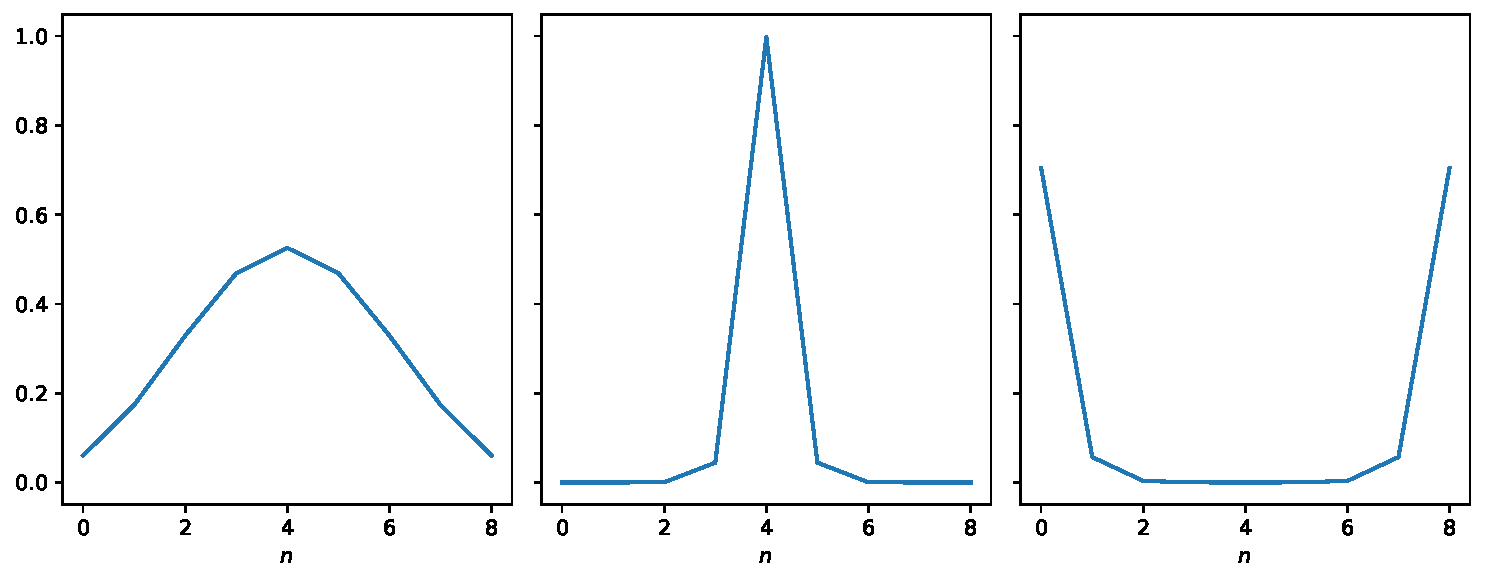
\includegraphics[width=.8\textwidth]{wf.pdf}
    \caption{Wave function}
    \label{3.9 fig wf}
\end{figure}

% density matrix
The density matrix are
\begin{minted}{text}
    [[0.004 0.01  0.02  0.028 0.032 0.028 0.02  0.01  0.004]
    [0.01  0.03  0.057 0.081 0.091 0.081 0.057 0.03  0.01 ]
    [0.02  0.057 0.108 0.154 0.173 0.154 0.108 0.057 0.02 ]
    [0.028 0.081 0.154 0.22  0.246 0.22  0.154 0.081 0.028]
    [0.032 0.091 0.173 0.246 0.276 0.246 0.173 0.091 0.032]
    [0.028 0.081 0.154 0.22  0.246 0.22  0.154 0.081 0.028]
    [0.02  0.057 0.108 0.154 0.173 0.154 0.108 0.057 0.02 ]
    [0.01  0.03  0.057 0.081 0.091 0.081 0.057 0.03  0.01 ]
    [0.004 0.01  0.02  0.028 0.032 0.028 0.02  0.01  0.004]]
   [[0.    0.    0.    0.    0.    0.    0.    0.    0.   ]
    [0.    0.    0.    0.    0.    0.    0.    0.    0.   ]
    [0.    0.    0.    0.    0.    0.    0.    0.    0.   ]
    [0.    0.    0.    0.002 0.044 0.002 0.    0.    0.   ]
    [0.    0.    0.    0.044 0.996 0.044 0.    0.    0.   ]
    [0.    0.    0.    0.002 0.044 0.002 0.    0.    0.   ]
    [0.    0.    0.    0.    0.    0.    0.    0.    0.   ]
    [0.    0.    0.    0.    0.    0.    0.    0.    0.   ]
    [0.    0.    0.    0.    0.    0.    0.    0.    0.   ]]
   [[0.497 0.04  0.003 0.    0.    0.    0.003 0.04  0.497]
    [0.04  0.003 0.    0.    0.    0.    0.    0.003 0.04 ]
    [0.003 0.    0.    0.    0.    0.    0.    0.    0.003]
    [0.    0.    0.    0.    0.    0.    0.    0.    0.   ]
    [0.    0.    0.    0.    0.    0.    0.    0.    0.   ]
    [0.    0.    0.    0.    0.    0.    0.    0.    0.   ]
    [0.003 0.    0.    0.    0.    0.    0.    0.    0.003]
    [0.04  0.003 0.    0.    0.    0.    0.    0.003 0.04 ]
    [0.497 0.04  0.003 0.    0.    0.    0.003 0.04  0.497]]
\end{minted}

% relative particle fluctuations
The relative particle fluctuations in three regimes are 
\begin{minted}{text}
    [7.863081011461077, 0.015831682417565402, 63.817067740969534]
\end{minted}
in first regime, $\braket{(\Delta \hat{N})^2} \approx  N$, in second regime, $\braket{(\Delta \hat{N})^2} \approx 0$, and in third regime, $\braket{(\Delta \hat{N})^2} \approx N^2$, which is consistent with the theoretically results.

% excitation gap
The excitation gap as a function of total particle number N is plotted as

\begin{figure}[h]
    \centering
    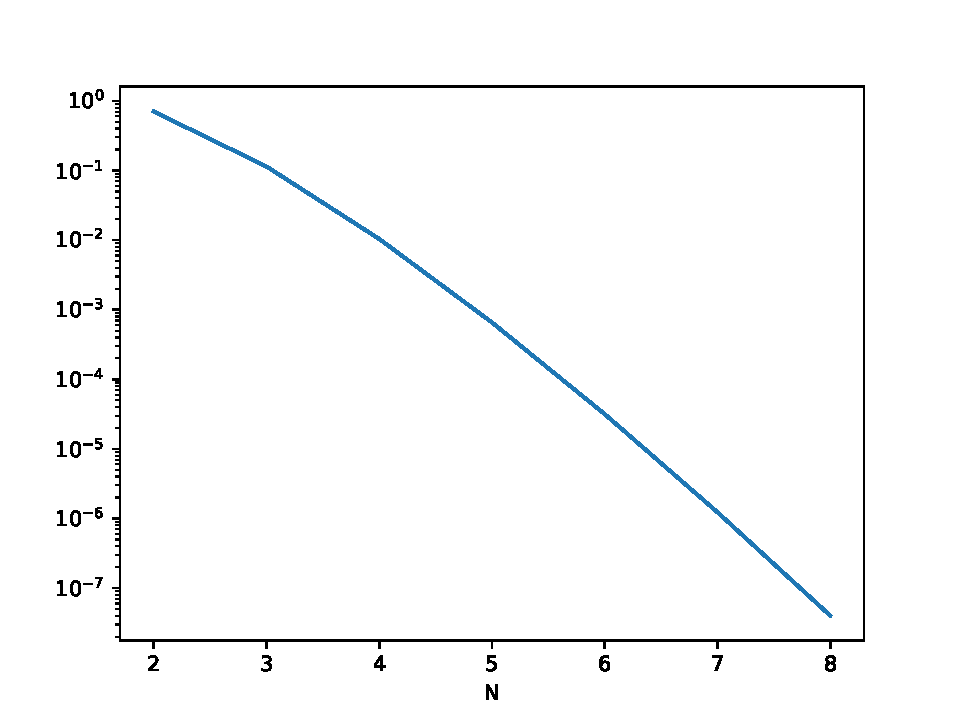
\includegraphics[width=.8\textwidth]{gap.pdf}
    \caption{Excitation gap}
    \label{3.9 fig gap}
\end{figure}

So as the number N increases, the excitation gap is close to zero, which means the ground state and the first excited state degenerate. While the ground state is symmetric and the first excited state is antisymmetric, this implies spontaneous symmetry breaking.
\section*{Problem 3.10}
Discuss the Hanbury-Brown-Twiss effect for noninteracting fermions and compare its difference with noninteracting bosons.
\paragraph*{Solution:}
We made two groups of noninteracting bosons and put them into the double-well, the initial state is given by 
\begin{equation}
    \ket{\Psi} = \frac{1}{\sqrt[]{(N/2)!}} \left(\hat{a}^{\dagger}_1 \hat{a}^{\dagger}_2\right)^{N/2} \ket{0} 
\end{equation}
With 
\begin{equation}
    \hat{\Psi}(\bm{r}) = \Psi_1(\bm{r}) \hat{a}_1 + \Psi_2(\bm{r}) \hat{a}_2
\end{equation}
the ensemble average of the density can be written as 
\begin{equation}
    n(\bm{r}) 
    = \braket{\hat{\Psi}^{\dagger}(\bm{r}) \hat{\Psi}(\bm{r})} 
    = \braket{\hat{a}^{\dagger}_1 \hat{a}_1} |\Psi_1(\bm{r})|^2
    + \braket{\hat{a}^{\dagger}_2 \hat{a}_2} |\Psi_2(\bm{r})|^2
\end{equation}
And the ensemble average of the density-density correlation is 
\begin{equation}
    \begin{aligned}
        \braket{\widetilde{n}(\bm{r}) \widetilde{n}(\bm{r}') } 
        &= \braket{\hat{\Psi}^{\dagger}(\bm{r}) \hat{\Psi}(\bm{r})\hat{\Psi}^{\dagger}(\bm{r}')\hat{\Psi}(\bm{r}')} \\
        &= n(\bm{r})n(\bm{r}') 
        + \braket{\hat{a}^{\dagger}_1 \hat{a}_1} \braket{\hat{a}^{\dagger}_2 \hat{a}_2} 
        \left(\Psi^*_1(\bm{r})\Psi^*_2(\bm{r}')\Psi_2(\bm{r})\Psi_1(\bm{r}')  + \mathrm{h.c.} \right)
    \end{aligned}
\end{equation}

For fermions, the initial state is
\begin{equation}
    \ket{\Psi} = \ket{1,1}
\end{equation}
and the correlation is 
\begin{equation}
    \begin{aligned}
        \braket{\widetilde{n}(\bm{r}) \widetilde{n}(\bm{r}') } 
        &= \braket{\hat{\Psi}^{\dagger}(\bm{r}) \hat{\Psi}(\bm{r})\hat{\Psi}^{\dagger}(\bm{r}')\hat{\Psi}(\bm{r}')}
        = n(\bm{r})n(\bm{r}') \\
        & + \braket{\hat{a}^{\dagger}_1 \hat{a}_1} (1- \braket{\hat{a}^{\dagger}_2 \hat{a}_2} )
        \left(\Psi^*_1(\bm{r})\Psi^*_2(\bm{r}')\Psi_2(\bm{r})\Psi_1(\bm{r}') \right) \\
        & + \braket{\hat{a}^{\dagger}_2 \hat{a}_2} (1- \braket{\hat{a}^{\dagger}_1 \hat{a}_1} )
        \left(\Psi_1(\bm{r})\Psi_2(\bm{r}')\Psi^*_2(\bm{r})\Psi^*_1(\bm{r}') \right)
    \end{aligned}
\end{equation}
because of $ \braket{\hat{a}^{\dagger}_i \hat{a}_i} = 1$, the last two terms in correlation both are zero. So there is no interference pattern for fermions.
\section*{Problem 6.1}
Solve the Cooper problem Eq.6.8 and compare the solution with the solution of the two-body problem in a vacuum of Eq.6.5 for positive $a_s$.
\paragraph*{Solution:}
In a vacuum, 
\begin{equation}
    \begin{aligned}
        \frac{m}{4\pi \hbar^2 a_s}
        & = \frac{1}{V} \sum_{\bm{k}} \left(\frac{1}{E - 2 \epsilon_{\bm{k}} } + \frac{1}{2 \epsilon_{\bm{k}}}\right)\\
        & =\frac{4\pi E}{V} \frac{V}{(2\pi)^3} \int_{0}^{\infty}  \,k^2 dk \frac{1}{\left(E - \frac{\hbar^2 k^2}{m}\right) \frac{\hbar^2 k^2}{m}} \\
        & = \frac{E}{2 \pi^2} \left(\frac{m}{\hbar^2}\right)^2
        \int_{0}^{\infty} \frac{dk}{\frac{mE}{\hbar^2} - k^2}
    \end{aligned}
\end{equation}
if $E>0$, we can infer from
\begin{equation}
    \int_{0}^{\infty} \frac{dx}{1 - x^2} 
    = \frac{1}{2} \left. \ln \frac{|1+x| }{|1-x| }\right \vert ^{\infty}_0
    = 0
\end{equation}
that $ \frac{m}{4\pi \hbar^2 a_s} = 0$, which also applies when $E = 0$.
When $E <0$, from
\begin{equation}
    \int_{0}^{\infty} \frac{dx}{a^2 + x^2}
    = \left.\frac{\arctan x/a}{a}\right \vert^{\infty}_0
    = \frac{\pi}{2a}
\end{equation}
we get
\begin{equation}
    \frac{m}{4\pi \hbar^2 a_s}
    = \frac{1}{4 \pi} \left(\frac{m}{\hbar^2}\right)^{3/2} \sqrt[]{-E}
\end{equation}
simplied as 
\begin{equation}
    E = - \frac{\hbar^2}{ma^2_s}
\end{equation}

On top of a Fermi sea, we have
\begin{equation}
    \begin{aligned}
        \frac{m}{4\pi \hbar^2 a_s}
        & = \frac{1}{V} \left[ \sum_{|\bm{k}| > k_F} \left(\frac{1}{E - 2 (\epsilon_{\bm{k}} - \mu) } + \frac{1}{2 \epsilon_{\bm{k}}}\right)\right] \\ 
        & = \frac{E+2\mu}{2\pi^2} \left(\frac{m}{\hbar^2}\right)^2
        \int_{k_F}^{\infty} \frac{dk}{\frac{m(E+2\mu)}{\hbar^2} - k^2}
        + \frac{1}{2\pi^2} \frac{m}{\hbar^2} \int_{0}^{k_F} dk
    \end{aligned}
\end{equation}

When $E > -2\mu$, we have
\begin{equation}
    \int_{k_F}^{\infty} \frac{dk}{\frac{m(E+2\mu)}{\hbar^2} - k^2}
    = \frac{1}{2} \left. \ln \frac{|\sqrt{\frac{mE}{\hbar^2}+k_F}+k| }{|\sqrt{\frac{mE}{\hbar^2}+k_F}-k| }\right \vert ^{\infty}_{k_F}
    = \frac{1}{2} \ln \frac{|\sqrt{\frac{mE}{\hbar^2}+k_F} - k_F| }{|\sqrt{\frac{mE}{\hbar^2}+k_F} + k_F| }
\end{equation}

When $E < -2\mu$, we have
\begin{equation}
    \begin{aligned}
        \int_{k_F}^{\infty} \frac{dk}{\frac{m(E+2\mu)}{\hbar^2} - k^2}
        & = - \left.
        \frac{1}{\sqrt{-m(E+2\mu)/\hbar^2}}    
        \arctan \frac{k}{\sqrt{-m(E+2\mu)/\hbar^2}}
        \right \vert^{\infty}_{k_F}\\
        & = \frac{1}{\sqrt{-m(E+2\mu)/\hbar^2}}
        (\frac{\pi}{2} - \arctan \frac{k_F}{\sqrt{-m(E+2\mu)/\hbar^2}})
    \end{aligned}
\end{equation}
take this back to the expression and then obtain the result.
\section*{Problem 6.2}
Calculate the ground state energy of the BCS mean-field Hamiltonian as a function of $\Delta $, and minimize this ground state energy with respect to $\Delta $ to obtain the gap equation.
\paragraph*{Solution:}
The mean-field Hamiltonian is 
\begin{equation}
    H_{BCS} 
    = \sum_{\bm{k}} \left[\mathcal{E}_{\bm{k}} 
    \left( \hat{\alpha}^{\dagger}_{\bm{k}} \hat{\alpha}_{\bm{k}} 
    + \hat{\beta}^{\dagger}_{\bm{k}}\hat{\beta}_{\bm{k}}\right) 
    + \left( \epsilon_{\bm{k}} - \mu\right)
    - \mathcal{E}_{\bm{k}} \right]
    - \frac{\Delta^2 V}{g}
\end{equation}
with 
\begin{equation}
    \mathcal{E}_{\bm{k}} = \sqrt{(\epsilon_{\bm{k}}-\mu)^2 + \Delta^2}
\end{equation}
For ground state, we have
\begin{equation}
    \hat{\alpha}_{\bm{k}} \ket{\Psi_{BCS}} = 0, \, 
    \hat{\beta}_{\bm{k}} \ket{\Psi_{BCS}} = 0
\end{equation}
so the ground state energy is given by 
\begin{equation}
    E_{BCS} = \sum_{\bm{k}} \left[
        (\epsilon_{\bm{k}} - \mu) - \mathcal{E}_{\bm{k}}
    \right] 
    - \frac{\Delta^2 V}{g}
\end{equation}
take the partial derivative of $E_{BCS}$ with respect to $\Delta$, we get 
\begin{equation}
    \frac{\partial E_{BCS}}{\partial \Delta}
    = \sum_{\bm{k}} \frac{\Delta}{\mathcal{E}_{\bm{k}}} - \frac{2\Delta V}{g} = 0
\end{equation}
and then we get
\begin{equation}
    \frac{1}{g} 
    = \frac{1}{V} \sum_{\bm{k}} \frac{1}{2 \mathcal{E}_{\bm{k}}}
\end{equation}
using the renormalizetion condition for g and we get 
\begin{equation}
    -\frac{m}{4\pi \hbar^2 a_s}
    = \frac{1}{V} \sum_{\bm{k}} \left(
        \frac{1}{2 \mathcal{E}_{\bm{k}}} 
        - \frac{1}{2 \epsilon_{\bm{k}}}
    \right)
\end{equation}
which is the gap equation. 
\section*{Problem 6.3}
Discuss the self-consistent solution of the BCS problem for the Hamiltonian
\begin{equation}
    H_{BCS} 
    = \sum_{\bm{k}, \sigma} (\epsilon_{\bm{k}} - \mu_{\sigma}) \hat{c}^{\dagger}_{\bm{k}\sigma} \hat{c}_{\bm{k}\sigma}
    + \sum_{\bm{k}} \Delta \hat{c}^{\dagger}_{\bm{k}\uparrow } \hat{c}^{\dagger}_{\bm{-k}\downarrow }
    + \sum_{\bm{k}} \Delta^* \hat{c}_{\bm{-k}\downarrow } \hat{c}_{\bm{k}\uparrow }
\end{equation}
when $\mu_{\uparrow} \neq \mu_{\downarrow}$, and compare the energy of the BCS state with the free Fermi gas for different $h = \mu_{\uparrow} - \mu_{\downarrow}$.
\paragraph*{Solution:}
This Hamiltonian is
\begin{equation}
    H_{BCS} 
    = \sum_{\bm{k}} \left[
        (\hat{c}^{\dagger}_{\bm{k}\uparrow } ,\, \hat{c}_{\bm{-k}\downarrow } )
        \begin{pmatrix}
            \epsilon_{\bm{k}} - \mu_{\uparrow} & \Delta \\
            \Delta^* & -(\epsilon_{\bm{k}} - \mu_{\downarrow})
        \end{pmatrix}
        \binom{\hat{c}_{\bm{k}\uparrow}}{\hat{c}^{\dagger}_{\bm{-k}\downarrow}}
        + (\epsilon_{\bm{k}} - \mu_{\downarrow})
    \right]
\end{equation}
which can be diagonalized as 
\begin{equation}
    H_{BCS}
    = \sum_{\bm{k}} \left[
        (\mathcal{E}_{\bm{k}} - \frac{h}{2}) 
        \hat{\alpha}^{\dagger}_{\bm{k}} \hat{\alpha}_{\bm{k}} 
        + (\mathcal{E}_{\bm{k}} + \frac{h}{2}) 
        \hat{\beta}^{\dagger}_{\bm{k}}\hat{\beta}_{\bm{k}}
        + \left( \epsilon_{\bm{k}} - \bar{\mu}\right)
        - \mathcal{E}_{\bm{k}}
    \right]
\end{equation}
with 
\begin{equation}
    \mathcal{E}_{\bm{k}} = \sqrt{(\epsilon_{\bm{k}}-\bar{\mu})^2 + \Delta^2}
\end{equation}
When $h<\Delta$, the ground is the same as the one with the same chemical potential, and the energy is 
\begin{equation}
    E_{BCS} = \sum_{\bm{k}} \left[
        (\epsilon_{\bm{k}} - \bar{\mu}) - \mathcal{E}_{\bm{k}}
    \right] 
\end{equation}


\end{document}